\documentclass{article}\usepackage[]{graphicx}\usepackage[]{color}
% maxwidth is the original width if it is less than linewidth
% otherwise use linewidth (to make sure the graphics do not exceed the margin)
\makeatletter
\def\maxwidth{ %
  \ifdim\Gin@nat@width>\linewidth
    \linewidth
  \else
    \Gin@nat@width
  \fi
}
\makeatother

\definecolor{fgcolor}{rgb}{0.345, 0.345, 0.345}
\newcommand{\hlnum}[1]{\textcolor[rgb]{0.686,0.059,0.569}{#1}}%
\newcommand{\hlstr}[1]{\textcolor[rgb]{0.192,0.494,0.8}{#1}}%
\newcommand{\hlcom}[1]{\textcolor[rgb]{0.678,0.584,0.686}{\textit{#1}}}%
\newcommand{\hlopt}[1]{\textcolor[rgb]{0,0,0}{#1}}%
\newcommand{\hlstd}[1]{\textcolor[rgb]{0.345,0.345,0.345}{#1}}%
\newcommand{\hlkwa}[1]{\textcolor[rgb]{0.161,0.373,0.58}{\textbf{#1}}}%
\newcommand{\hlkwb}[1]{\textcolor[rgb]{0.69,0.353,0.396}{#1}}%
\newcommand{\hlkwc}[1]{\textcolor[rgb]{0.333,0.667,0.333}{#1}}%
\newcommand{\hlkwd}[1]{\textcolor[rgb]{0.737,0.353,0.396}{\textbf{#1}}}%
\let\hlipl\hlkwb

\usepackage{framed}
\makeatletter
\newenvironment{kframe}{%
 \def\at@end@of@kframe{}%
 \ifinner\ifhmode%
  \def\at@end@of@kframe{\end{minipage}}%
  \begin{minipage}{\columnwidth}%
 \fi\fi%
 \def\FrameCommand##1{\hskip\@totalleftmargin \hskip-\fboxsep
 \colorbox{shadecolor}{##1}\hskip-\fboxsep
     % There is no \\@totalrightmargin, so:
     \hskip-\linewidth \hskip-\@totalleftmargin \hskip\columnwidth}%
 \MakeFramed {\advance\hsize-\width
   \@totalleftmargin\z@ \linewidth\hsize
   \@setminipage}}%
 {\par\unskip\endMakeFramed%
 \at@end@of@kframe}
\makeatother

\definecolor{shadecolor}{rgb}{.97, .97, .97}
\definecolor{messagecolor}{rgb}{0, 0, 0}
\definecolor{warningcolor}{rgb}{1, 0, 1}
\definecolor{errorcolor}{rgb}{1, 0, 0}
\newenvironment{knitrout}{}{} % an empty environment to be redefined in TeX

\usepackage{alltt}

% utf8 characters
\usepackage[utf8]{inputenc}

% maths
\usepackage{amsfonts}
\usepackage{amsmath}
\usepackage{amssymb}
\usepackage{amsthm}
\newtheorem{theorem}{Theorem}
\DeclareMathOperator*{\argmax}{arg\,max}
\DeclareMathOperator*{\argmin}{arg\,min}

% bold math
\usepackage{bm}
% The following remaps \boldsymbol and \mathbf to \bm
\renewcommand{\boldsymbol}[1]{\bm{#1}}
\renewcommand{\mathbf}[1]{\bm{#1}}

% graphics
\usepackage{graphicx}

\renewcommand{\baselinestretch}{1}

\title{linearAlgebra: Benchmarks}
\author{Ivan Jacob Agaloos Pesigan}
\date{}
\IfFileExists{upquote.sty}{\usepackage{upquote}}{}
\begin{document}

\maketitle





\section{.center}



\begin{knitrout}
\definecolor{shadecolor}{rgb}{0.969, 0.969, 0.969}\color{fgcolor}\begin{kframe}
\begin{verbatim}
#> Unit: microseconds
#>   expr     min      lq      mean   median      uq      max neval
#>     .d  18.273  54.201  73.47216  56.0805  58.555 4626.714   500
#>  scale 105.513 174.854 180.57393 177.7710 183.171  508.355   500
\end{verbatim}


{\ttfamily\noindent\itshape\color{messagecolor}{\#> Coordinate system already present. Adding new coordinate system, which will replace the existing one.}}\begin{verbatim}
#> [[1]]
\end{verbatim}
\end{kframe}
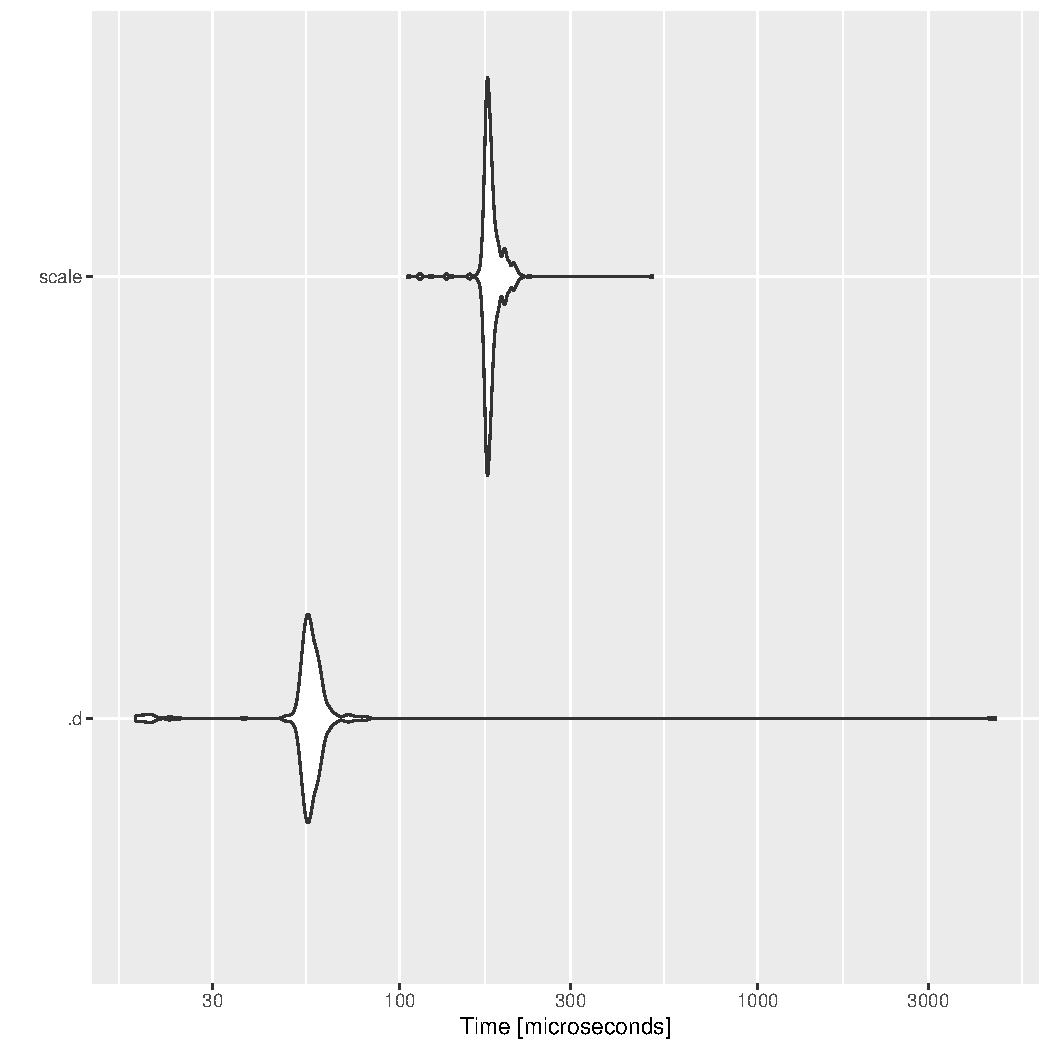
\includegraphics[width=1\linewidth]{man/figures/latex-test-benchmark-linearAlgebra-d-dot-1} 

\end{knitrout}

\newpage

\section{.deltacapsq}



\begin{knitrout}
\definecolor{shadecolor}{rgb}{0.969, 0.969, 0.969}\color{fgcolor}\begin{kframe}
\begin{verbatim}
#> Unit: microseconds
#>         expr     min       lq     mean   median       uq      max neval
#>  .deltacapsq  76.191  78.9535 101.9013  82.0450  89.1695 1651.408   500
#>  mahalanobis 208.980 217.1905 289.7014 224.1595 255.6505 3230.357   500
\end{verbatim}


{\ttfamily\noindent\itshape\color{messagecolor}{\#> Coordinate system already present. Adding new coordinate system, which will replace the existing one.}}\begin{verbatim}
#> [[1]]
\end{verbatim}
\end{kframe}
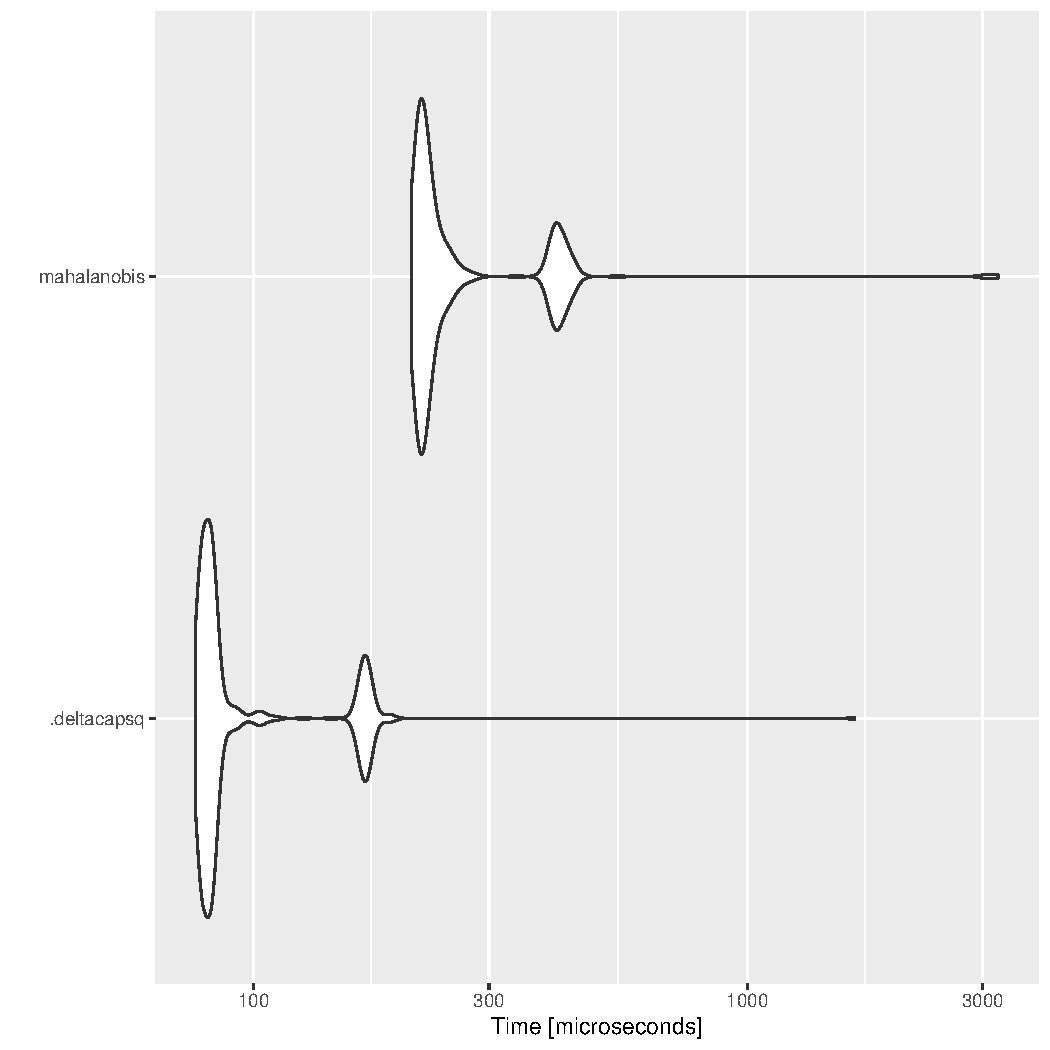
\includegraphics[width=1\linewidth]{man/figures/latex-test-benchmark-linearAlgebra-deltacapsq-dot-1} 

\end{knitrout}

\newpage

\section{.pinv\_of\_dcap}



\begin{knitrout}
\definecolor{shadecolor}{rgb}{0.969, 0.969, 0.969}\color{fgcolor}\begin{kframe}
\begin{verbatim}
#> Unit: microseconds
#>           expr    min      lq      mean  median      uq      max neval
#>  .pinv_of_dcap  7.623  7.9955  8.752116  8.5600  8.8750   53.539   500
#>     MASS::ginv 26.038 26.6940 41.466082 27.0285 27.5035 7036.737   500
\end{verbatim}


{\ttfamily\noindent\itshape\color{messagecolor}{\#> Coordinate system already present. Adding new coordinate system, which will replace the existing one.}}\begin{verbatim}
#> Unit: microseconds
#>           expr    min     lq     mean  median      uq     max neval
#>  .pinv_of_dcap  8.508  8.901  9.91210  9.7990 10.2095  53.499   500
#>     MASS::ginv 27.845 28.928 30.22158 29.4475 30.0435 120.228   500
\end{verbatim}


{\ttfamily\noindent\itshape\color{messagecolor}{\#> Coordinate system already present. Adding new coordinate system, which will replace the existing one.}}\begin{verbatim}
#> Unit: microseconds
#>           expr    min      lq     mean median     uq     max neval
#>  .pinv_of_dcap 10.414 11.0375 12.13127 11.839 12.433  64.889   500
#>     MASS::ginv 30.402 31.9330 33.14095 32.523 33.230 105.038   500
\end{verbatim}


{\ttfamily\noindent\itshape\color{messagecolor}{\#> Coordinate system already present. Adding new coordinate system, which will replace the existing one.}}\begin{verbatim}
#> [[1]]
\end{verbatim}
\end{kframe}
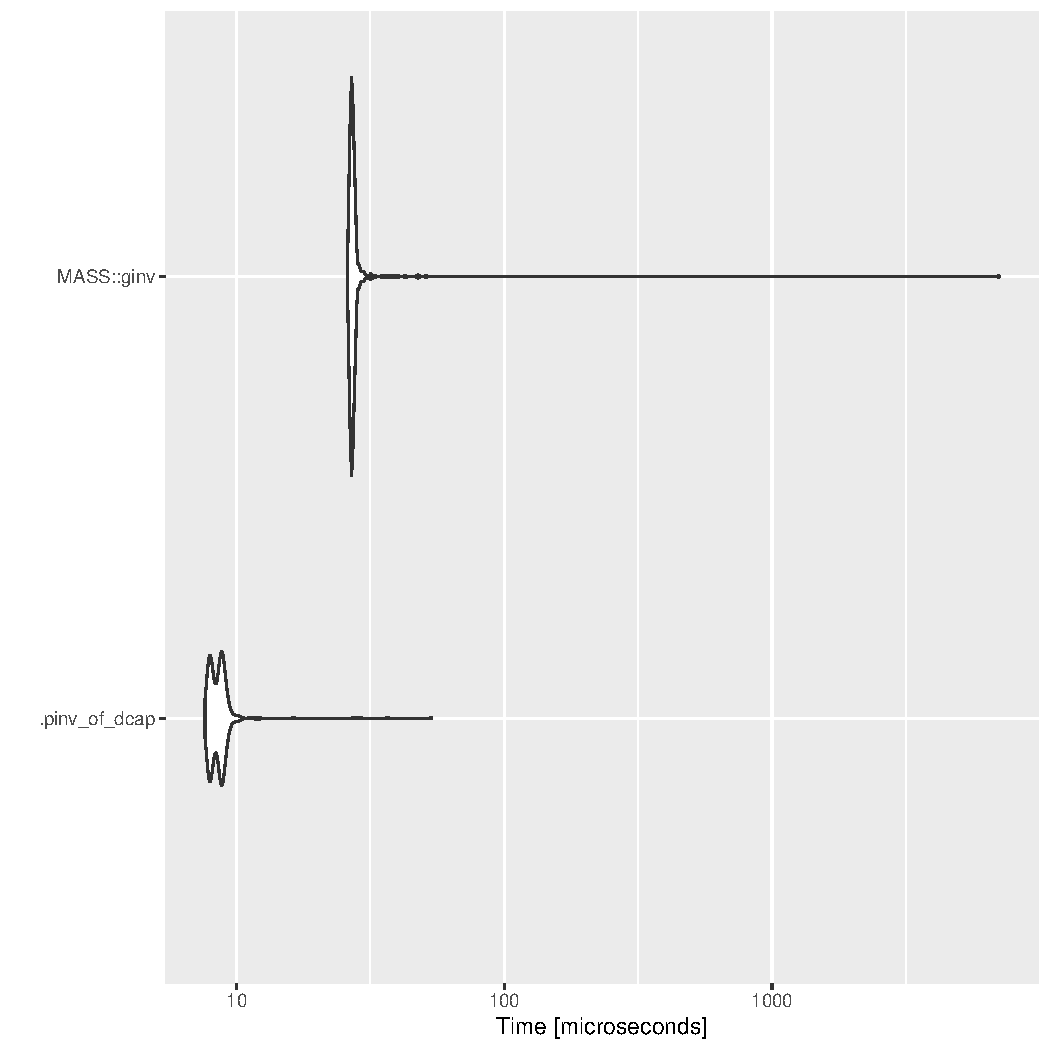
\includegraphics[width=1\linewidth]{man/figures/latex-test-benchmark-linearAlgebra-pinv-of-dcap-dot-1} 
\begin{kframe}\begin{verbatim}
#> 
#> [[2]]
\end{verbatim}
\end{kframe}
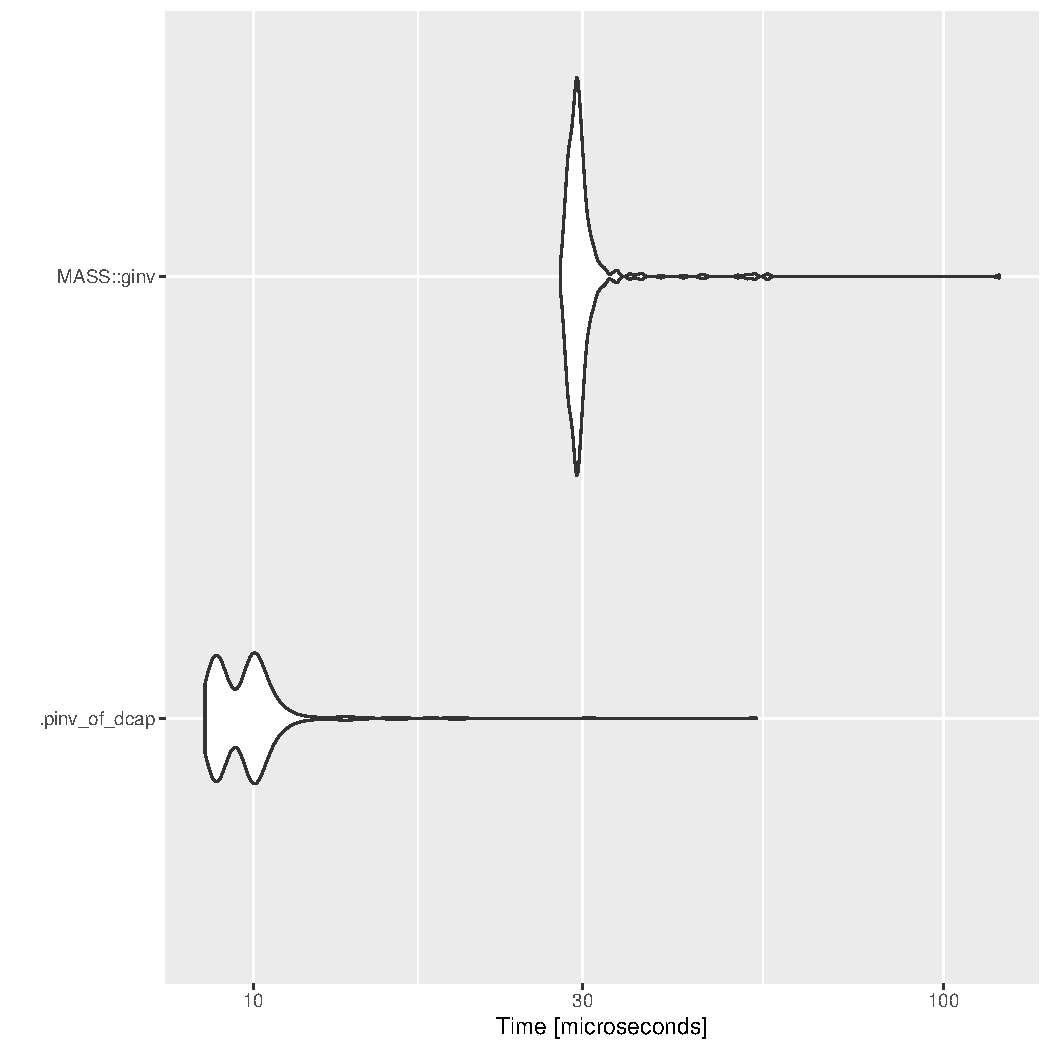
\includegraphics[width=1\linewidth]{man/figures/latex-test-benchmark-linearAlgebra-pinv-of-dcap-dot-2} 
\begin{kframe}\begin{verbatim}
#> 
#> [[3]]
\end{verbatim}
\end{kframe}
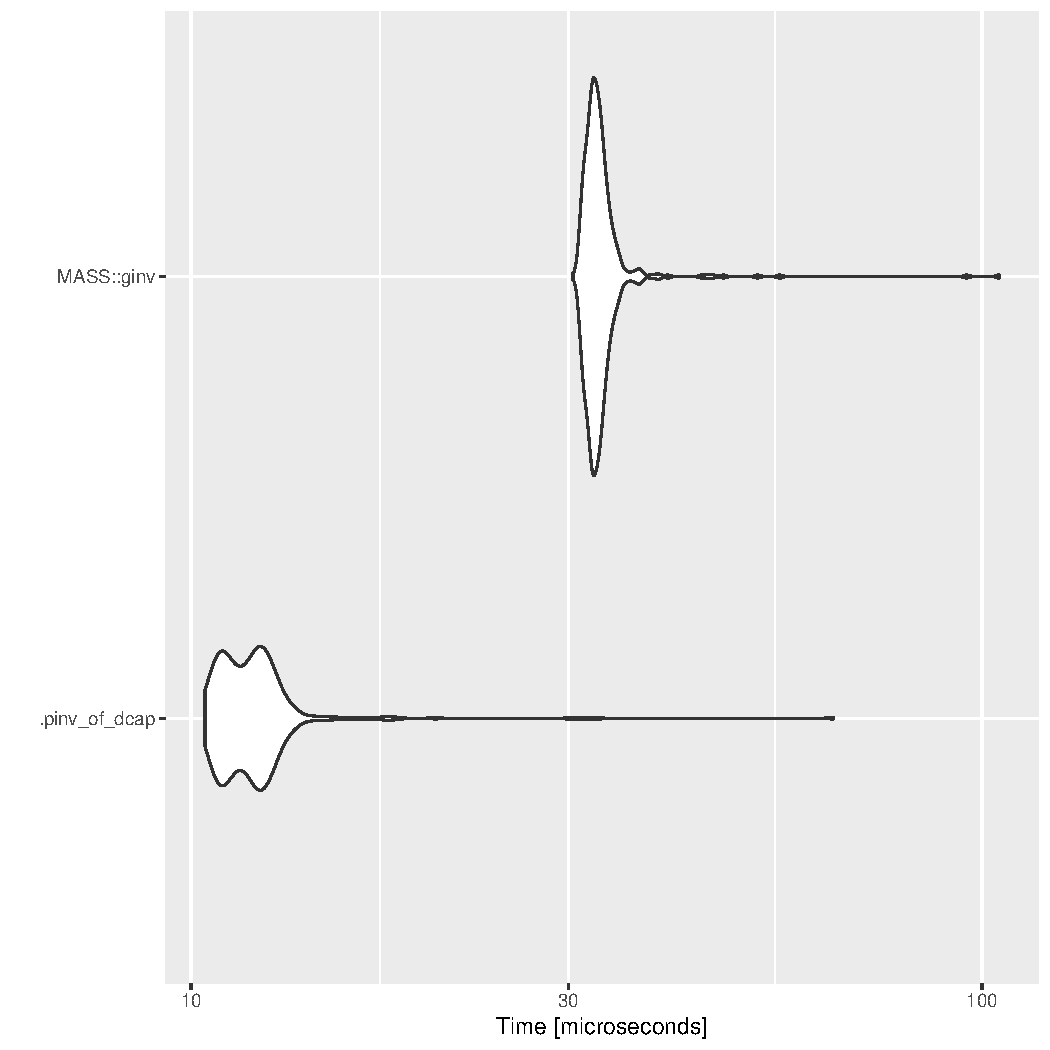
\includegraphics[width=1\linewidth]{man/figures/latex-test-benchmark-linearAlgebra-pinv-of-dcap-dot-3} 

\end{knitrout}

\newpage

\section{.vec}



\begin{knitrout}
\definecolor{shadecolor}{rgb}{0.969, 0.969, 0.969}\color{fgcolor}\begin{kframe}
\begin{verbatim}
#> Unit: nanoseconds
#>       expr     min      lq        mean  median      uq      max neval
#>       .vec     548    1301    5747.746    6807    8505    16019   500
#>          c 1757500 5062654 4755339.340 5256222 5308490 69536092   500
#>  as.vector 1257044 4549434 4064055.644 4639987 4694491  8473168   500
\end{verbatim}


{\ttfamily\noindent\itshape\color{messagecolor}{\#> Coordinate system already present. Adding new coordinate system, which will replace the existing one.}}\begin{verbatim}
#> [[1]]
\end{verbatim}
\end{kframe}
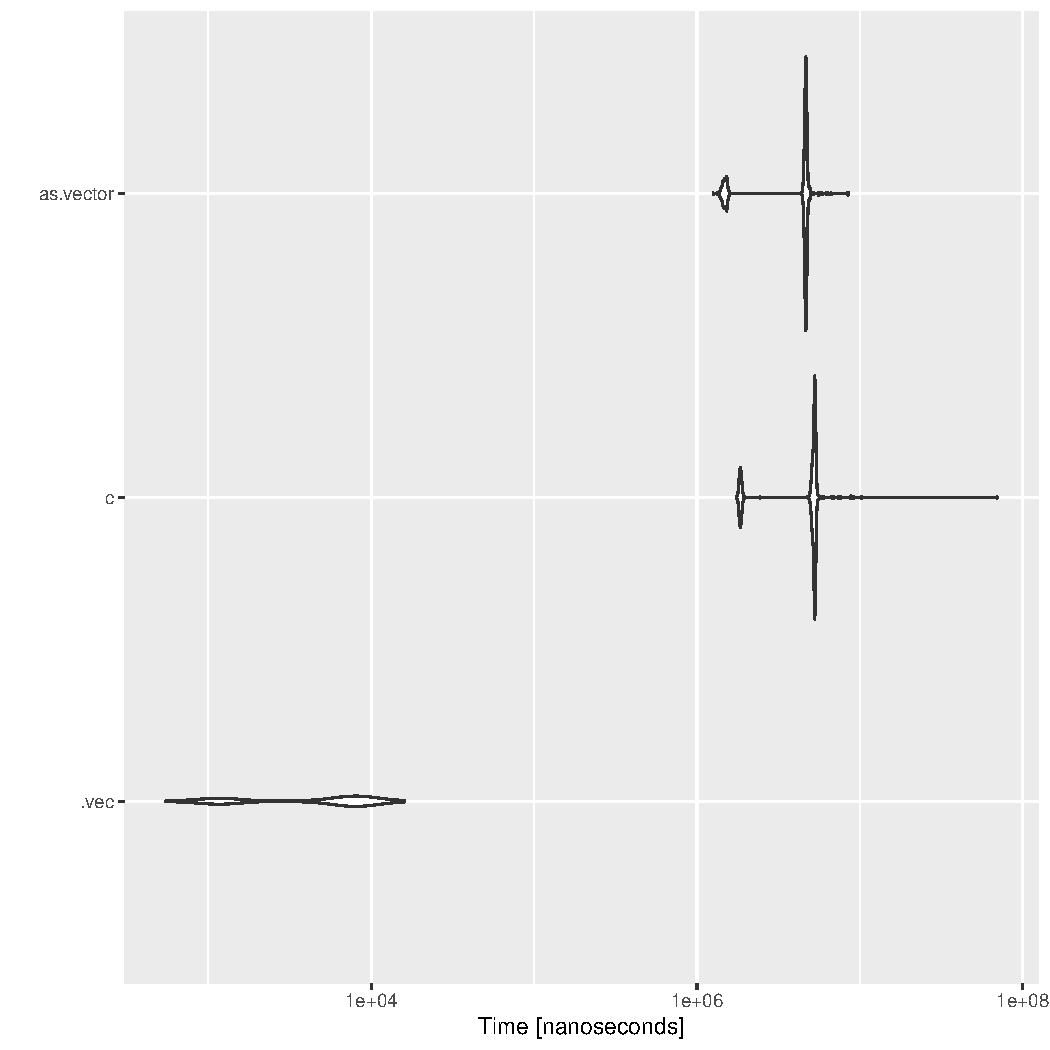
\includegraphics[width=1\linewidth]{man/figures/latex-test-benchmark-linearAlgebra-vec-dot-1} 

\end{knitrout}

\newpage

\section{.vec\_mean}



\begin{knitrout}
\definecolor{shadecolor}{rgb}{0.969, 0.969, 0.969}\color{fgcolor}\begin{kframe}
\begin{verbatim}
#> Unit: microseconds
#>       expr    min      lq     mean  median      uq      max neval
#>  .vec_mean  8.991  9.0830 12.25630  9.1270  9.1995 1496.100   500
#>   vec_mean  9.545  9.6690 14.80328  9.7415  9.8390 2481.583   500
#>       mean 19.093 19.2215 19.48147 19.2960 19.4655   37.309   500
\end{verbatim}


{\ttfamily\noindent\itshape\color{messagecolor}{\#> Coordinate system already present. Adding new coordinate system, which will replace the existing one.}}\begin{verbatim}
#> [[1]]
\end{verbatim}
\end{kframe}
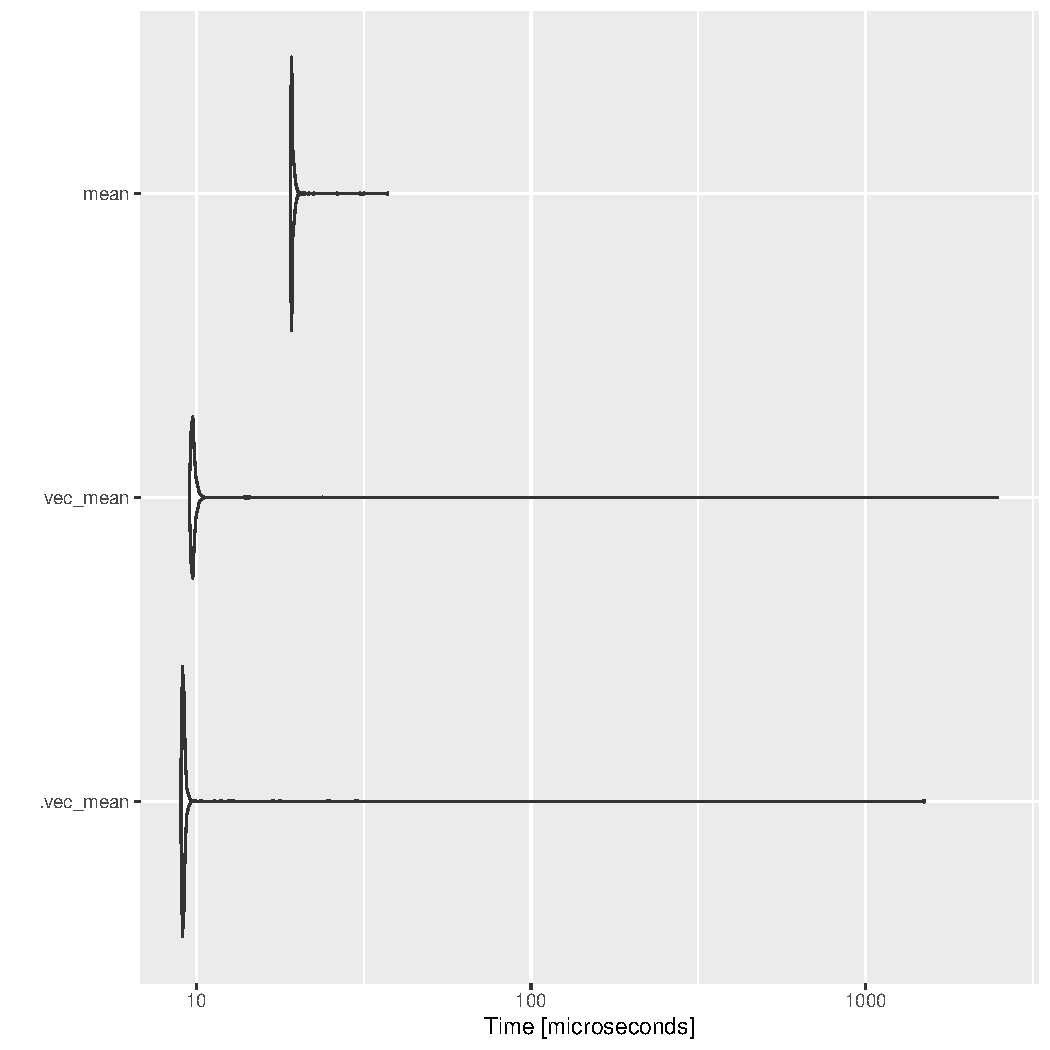
\includegraphics[width=1\linewidth]{man/figures/latex-test-benchmark-linearAlgebra-vec-mean-dot-1} 

\end{knitrout}

\newpage

\section{.z}



\begin{knitrout}
\definecolor{shadecolor}{rgb}{0.969, 0.969, 0.969}\color{fgcolor}\begin{kframe}
\begin{verbatim}
#> Unit: microseconds
#>   expr     min       lq      mean  median       uq      max neval
#>     .z  24.660  25.9510  37.36305  27.490  29.2005 3395.239   500
#>  scale 378.782 390.8935 451.00311 398.532 410.4730 3953.361   500
\end{verbatim}


{\ttfamily\noindent\itshape\color{messagecolor}{\#> Coordinate system already present. Adding new coordinate system, which will replace the existing one.}}\begin{verbatim}
#> [[1]]
\end{verbatim}
\end{kframe}
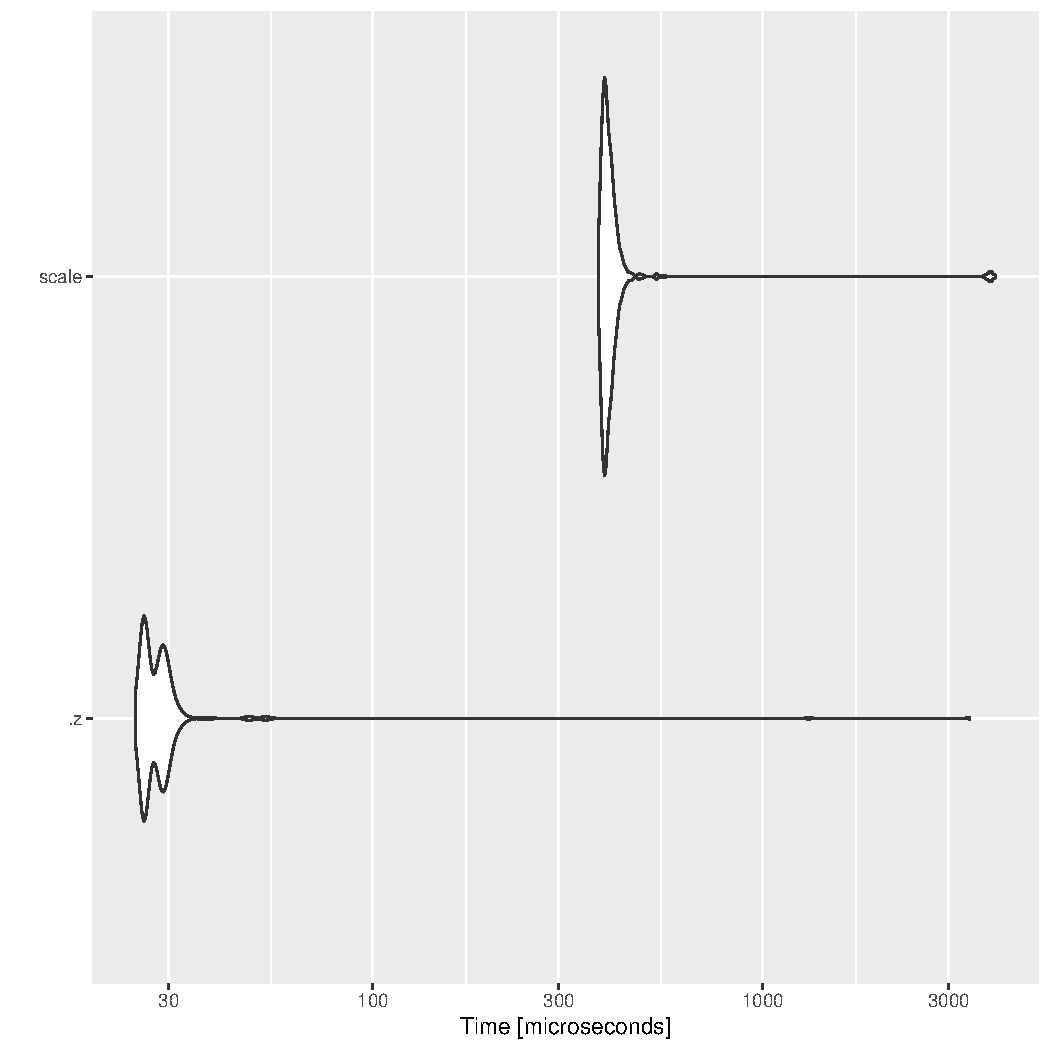
\includegraphics[width=1\linewidth]{man/figures/latex-test-benchmark-linearAlgebra-z-dot-1} 

\end{knitrout}

\newpage 

\section*{Environment}

\begin{knitrout}
\definecolor{shadecolor}{rgb}{0.969, 0.969, 0.969}\color{fgcolor}\begin{kframe}
\begin{alltt}
\hlkwd{ls}\hlstd{()}
\end{alltt}
\begin{verbatim}
#> [1] "FUN"  "i"    "root"
\end{verbatim}
\end{kframe}
\end{knitrout}

\section*{Class}

\begin{knitrout}
\definecolor{shadecolor}{rgb}{0.969, 0.969, 0.969}\color{fgcolor}\begin{kframe}
\begin{alltt}
\hlstd{obj_i} \hlkwb{<-} \hlkwd{lapply}\hlstd{(}
  \hlkwc{X} \hlstd{=} \hlkwd{ls}\hlstd{(),}
  \hlkwc{FUN} \hlstd{=} \hlkwa{function}\hlstd{(}\hlkwc{x}\hlstd{)} \hlkwd{eval}\hlstd{(}\hlkwd{parse}\hlstd{(}\hlkwc{text} \hlstd{= x))}
\hlstd{)}
\hlkwd{unique}\hlstd{(}
  \hlkwd{lapply}\hlstd{(}
    \hlkwc{X} \hlstd{= obj_i,}
    \hlkwc{FUN} \hlstd{= class}
  \hlstd{)}
\hlstd{)}
\end{alltt}
\begin{verbatim}
#> [[1]]
#> [1] "function"
#> 
#> [[2]]
#> [1] "character"
#> 
#> [[3]]
#> [1] "root_criterion"
\end{verbatim}
\end{kframe}
\end{knitrout}

\newpage

\section*{Session - Overleaf}

\begin{knitrout}
\definecolor{shadecolor}{rgb}{0.969, 0.969, 0.969}\color{fgcolor}\begin{kframe}
\begin{alltt}
\hlkwd{sessionInfo}\hlstd{()}
\end{alltt}
\begin{verbatim}
#> R version 4.1.2 (2021-11-01)
#> Platform: x86_64-pc-linux-gnu (64-bit)
#> Running under: Ubuntu 20.04.3 LTS
#> 
#> Matrix products: default
#> BLAS:   /usr/lib/x86_64-linux-gnu/atlas/libblas.so.3.10.3
#> LAPACK: /usr/lib/x86_64-linux-gnu/atlas/liblapack.so.3.10.3
#> 
#> locale:
#>  [1] LC_CTYPE=C.UTF-8       LC_NUMERIC=C           LC_TIME=C.UTF-8       
#>  [4] LC_COLLATE=C.UTF-8     LC_MONETARY=C.UTF-8    LC_MESSAGES=C.UTF-8   
#>  [7] LC_PAPER=C.UTF-8       LC_NAME=C              LC_ADDRESS=C          
#> [10] LC_TELEPHONE=C         LC_MEASUREMENT=C.UTF-8 LC_IDENTIFICATION=C   
#> 
#> attached base packages:
#> [1] stats     graphics  grDevices utils     datasets  methods   base     
#> 
#> loaded via a namespace (and not attached):
#>  [1] knitr_1.36           magrittr_2.0.1       MASS_7.3-54         
#>  [4] munsell_0.5.0        colorspace_2.0-2     R6_2.5.1            
#>  [7] rlang_0.4.12         fansi_0.5.0          stringr_1.4.0       
#> [10] highr_0.9            tools_4.1.2          grid_4.1.2          
#> [13] gtable_0.3.0         xfun_0.28            tinytex_0.35        
#> [16] utf8_1.2.2           ellipsis_0.3.2       digest_0.6.29       
#> [19] rprojroot_2.0.2      tibble_3.1.6         lifecycle_1.0.1     
#> [22] crayon_1.4.2         farver_2.1.0         ggplot2_3.3.5       
#> [25] microbenchmark_1.4.9 vctrs_0.3.8          glue_1.5.1          
#> [28] evaluate_0.14        stringi_1.7.6        compiler_4.1.2      
#> [31] pillar_1.6.4         scales_1.1.1         pkgconfig_2.0.3
\end{verbatim}
\end{kframe}
\end{knitrout}

\nocite{R-2021}

\printbibliography

\end{document}
